\documentclass[10pt]{beamer}

% --- Packages ---
\usepackage{graphicx}
\usepackage{booktabs} % For better looking tables
\usepackage{fontspec} % Tectonic-specific fix for font
\usepackage{tabularx}
\usepackage{array}
\newcolumntype{Y}{>{\raggedleft\arraybackslash}X}

% --- Presentation Settings ---
\usetheme{default}
\usecolortheme{seagull}
\usefonttheme{professionalfonts}

\title[Bachelor’s thesis Presentation]{Local LLM-based Terminal Assistant}
\subtitle{Bachelor’s thesis}
\author[Ostap Pelekh]{Author: Ostap Pelekh\\Supervizor: Ing. Roderik Ploszek, PhD.}
\institute[Slovak University of Technology in Bratislava]{Faculty of electrical engineering and information technology (FEI)}
\date[]{}

\begin{document}

% Xs Slide 1: Title Page
\begin{frame}
    \titlepage
\end{frame}

% Xs Slide 2: ToC
\begin{frame}
    \frametitle{Presentation outline}
    \begin{itemize}
        \item Introduction
            \begin{itemize}
                \item Thesis topic and racionale
                \item Theory
            \end{itemize}
        \item Thesis work
             \begin{itemize}
                 \item Approaches outline
                 \item Architecture outline
                 \item Classifier
                 \item Agentic
                 \item RAG
                 \item Latency tests
             \end{itemize}
        \item Conclusion
        \item Future work
        % \item \textbf{End}         % 18
    \end{itemize}
\end{frame}

% Xs Slide 3: Introduction + Racionale + What will be done pt.1 (just topic)
\begin{frame}
    \frametitle{Introduction: Thesis topic and racionale}
    \begin{itemize}
        \item \textbf{Objective}: test the use of local LLMs in the context of a terminal assistant
    \vspace{0.5cm} \small
        \item \textbf{Racionale}: offline execution, independence from remote
            servers, network access, privacy
        \item \textbf{Work overview}: this work has tested and evaluated different approaches
            for usage of local LLMs in the context of a terminal assistant. It
            also provides a reference implementation of such an assistant,
            avalable on GitHub (\texttt{Ostap4ello/shAI-l}) and university archive along
            % TODO: add link GH
            with the testing data and results.
    \vspace{0.5cm} \normalsize
    \item \textbf{Limitations}: usage of local LLMs under 2B parameters (suitable
        for devices with 8GB RAM)
    \end{itemize}
\end{frame}

% Xs Slide 4: Theory (main things)
\begin{frame}
    \frametitle{Introduction: Theory}
    \begin{itemize}
        \item terminal, shell, CLI, terminal applications, Bash
        \item language models, LLMs, embedding LLMs
        \item RAG, MRR, precision@k
        \item embeddings, vector databases, documents, man pages, top\_k
        \item AI/LLM agents
    \end{itemize}
\end{frame}

% Xs Slide 5: What will be done pt.2 (approaches desc)
\begin{frame}
    \frametitle{Approaches tested and evaluated}
    \begin{itemize}
        \item \textbf{Bash Integration \& Classifier}: Bash vs Natural Language Query, LLM-based
        \item \textbf{Agentic}: LLM agent naive approach, LLM-based
        \item \textbf{RAG}: Document database with vector embeddings with LLM
            summarization, LLM-based and embedding-LLM-based
    \vspace{0.5cm}
        \item \textbf{Application latency}: to provide a reference for user-experience
            and usability evaluation
    \end{itemize}
\end{frame}

% Xs Slide 6: What will be done pt.3 (app architecture)
\begin{frame}
    \frametitle{Architecture outline}
    \begin{itemize}
        \small
        \item \textbf{Core}: a two layered structure: % add image?
            \begin{itemize}
                \item Tools(low-level): DB, LLM and embedding LLM, utils, config
                \item Workflows(high-level): Classifier, RAG
            \end{itemize}
        \item \textbf{Interfaces}: application implements a CLI and programmatic API
            The CLI interface accesses both the workflows and the tools directly.
    \end{itemize}
    \begin{figure}[ht]
        \centering
        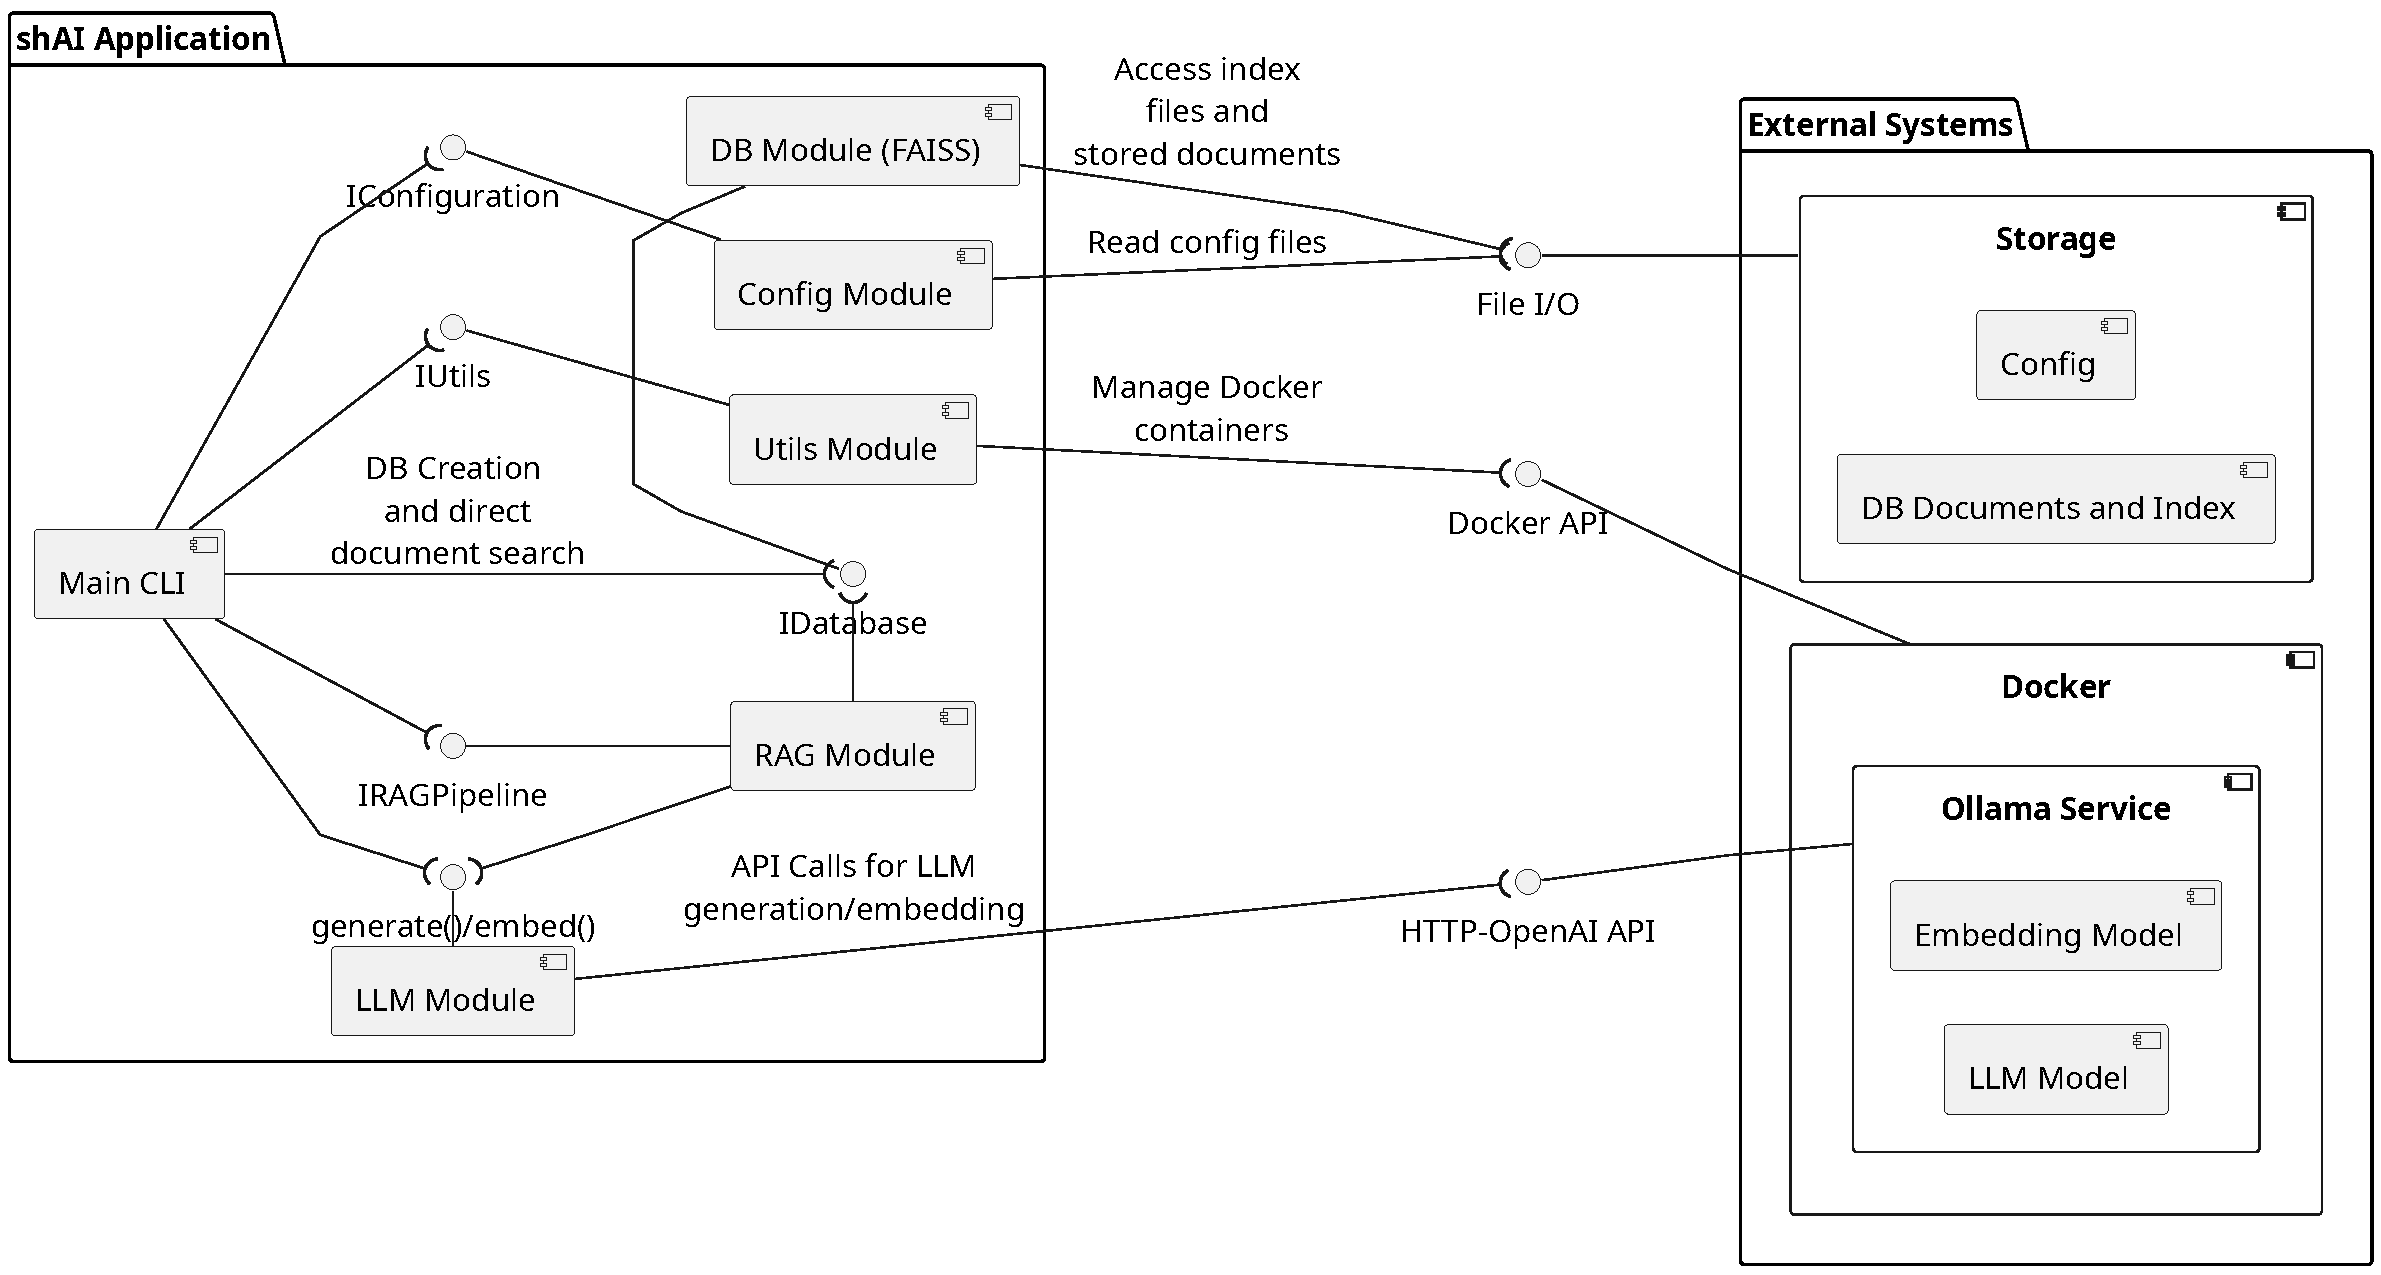
\includegraphics[width=0.8\textwidth]{res/component.puml.pdf}
        \caption{Component architecture of ShAI}\label{fig:component-arch}
    \end{figure}
\end{frame}

% Xs Slide 7: Classifier (idea+testing+results)
\begin{frame}
    \frametitle{Bash Integration \& Classifier}
    \begin{itemize}
        \item \textbf{Idea}: build a shell wrapper, which will behave either as
            chat or as a normal shell, depending on the user query, using a
            LLM-based classifier. This would blend the two modes of interaction
            and provide a unique seamless interface.
        \item \textbf{Testing}: \texttt{classifier-100} contains 100 inputs with
            a balanced mix of natural language queries and shell command inputs
            (e.g. ``How do I list files in a directory?'', ``ls -la
            /home/user'')
    \end{itemize}
\end{frame}

% Xs Slide 8: Classifier pt.2 (idea+testing+results)
\begin{frame}
    \frametitle{Bash Integration \& Classifier}

    \begin{table}[h]
      \centering
      \scriptsize
      \caption{Binary classification results on \texttt{classifier-100}.}
        \begin{tabular}{lrr}
        \toprule
        \textbf{Model} & \textbf{Accuracy} & \textbf{Avg Latency (s)} \\
        \midrule
        ibm/granite3.1-moe:1b & 53.0\% & 0.278 \\
        ibm/granite3.1-moe:3b & 60.0\% & 0.101 \\
        ibm/granite3.1-dense:2b & 83.0\% & 0.377 \\
        qwen3:0.6b & 79.0\% & 1.183 \\
        qwen3:1.7b & 88.0\% & 2.871 \\
        qwen2.5:0.5b & 50.0\% & 0.180 \\
        qwen2.5:1.5b & 78.0\% & 0.150 \\
        gemma3:1b & 65.0\% & 0.233 \\
        \bottomrule % TODO: lat?!
      \end{tabular}\label{tab:eval-classifier-results}
    \end{table}

    \begin{itemize}
        \item \textbf{Outcomes}: for a shell wrapper, the models have shown the
            following limitations:
            \begin{itemize}
                \item Low accuracy
                \item Unacceptable Latency for interactive use
                \item Complicated shell integration and maintenance
            \end{itemize}
            This component remains a \textbf{proof-of-concept} and was not
            pursued further.
    \end{itemize}
\end{frame}

% Xs Slide 9: Agentic (idea+testing+results) -- short
\begin{frame}
    \frametitle{Agentic approach}
    \begin{itemize}
        \item \textbf{Idea}: implement and test a classic agentic approach
        \item \textbf{Testing}: left in state of manual testing due to
            unreliability of the approach with the chosen models and constraints
        \item \textbf{Outcomes}: proved unreliable within the chosen constraints
            \textit{(but will be further mentioned in the future work)}
    \end{itemize}
\end{frame}

% Xs Slide 10: RAG pt.1 (idea+testing+results)
\begin{frame}
    \frametitle{RAG approach}
    \begin{itemize}
        \item \textbf{Idea}: implement a RAG-based workflow (DB module and
            LLM-based summarization) and test it within the constraints set.
            Three approaches were tested:
            \begin{itemize}
                \item Document-level retrieval
                \item Document retrieval with passage-level re-ranking
                  \textit{(retrieving documents first, then re-ranking passages
                    within them, evaluating by passage matches)}
                \item Passage-scope retrieval
            \end{itemize}
        \item \textbf{Testing}: tested DB retrieval MRR and precision@k on a
            collection of documents against reference queries and target lines
            on two collections:
            \begin{itemize}
              \item \texttt{sample-10}: 14 documents, 250 queries
              \item \texttt{sample-100}: 101 documents, 300 queries
            \end{itemize}
    \end{itemize}
\end{frame}

% Xs Slide 11: RAG pt.2 (results+conclusion)
\begin{frame}
  \frametitle{RAG approach}

  \begin{table}
    \small
    \centering
    \caption{Summary of embedding models used in experiments
    (dimension and context).}\label{tab:embedding-summary}
    \begin{tabularx}{\textwidth}{Xlll}
      \toprule
      \textbf{Model} & \textbf{Params} & \textbf{Context} &
      \textbf{Vector dim} \\
      \midrule
      Qwen3-Embedding-0.6B & 0.6B & 32K & up to 1024 \\
      EmbeddingGemma-300M (Google) & 300M & 2048 & 768 \\
      granite-embedding-30m-english & 30M & 512 & 384 \\
      granite-embedding-278m-multilingual & 278M & 512 & 768 \\
      \bottomrule
    \end{tabularx}
  \end{table}

\end{frame}

% Xs Slide 11: RAG pt.2 (results+conclusion)
\begin{frame}
    \frametitle{RAG approach}
\begin{table}[h]
  \centering
  \scriptsize
  \caption{Overview of Min/Max performance ranges across retrieval approaches on \texttt{sample-100}.}
  \begin{tabularx}{\textwidth}{llllYYY}
    \toprule
    \textbf{Approach}    & \textbf{Top-1} & \textbf{Top-5} & \textbf{MRR} & \textbf{Avg Latency (s)} & \textbf{Index Build (s)} & \textbf{Response Size (chars)} \\
    \midrule
    \textbf{Doc.}     & 62.7--72.7\% & 84.0--92.0\%  & 0.724--0.806 & 0.036--0.098 & 1.6--128.2  & 62--127K \\
    \textbf{Re-rank.} & 42.7--45.7\% & 72.7--79.7\%  & 0.530--0.571 & 0.595--3.745 & 2.1--128.5  & 6K        \\
    \textbf{Sec.}     & 67.3--69.0\% & 87.0--91.0\%  & 0.746--0.771 & 0.040--0.109 & 10.8--44.7  & 3K        \\
    \bottomrule
  \end{tabularx}\label{tab:overview-by-approach-scale}
\end{table}
    \begin{itemize}
        \item \textbf{Outcomes}:
            \begin{itemize}
                \item Robust accuracy with for all approaches
                \item Generated output size: secound and third approaches
                    allowed to reduce and control output sizes
                \item Latency: The first and third approaches had lower
                    retrieval latency (avg. 0.5--1.5s) than the second approach
                    (avg. 2--3.5s), due to in-runtime reranking. Document-level
                    indexing cause high latencies when embedding big files.
            \end{itemize}
    \end{itemize}
\end{frame}

% Xs Slide 12: Latency tests pt.1 (testing+results)
\begin{frame}
    \frametitle{Latency tests}
    \begin{itemize}
        \item \textbf{Idea}: test the latency of the application with different
            setups and approaches to provide a reference for user-experience and
            usability evaluation
        \item \textbf{Testing}: a set of scenarios for the whole system
            was created and tested with different setups, including: RAG and DB
            retrieval, index build times for different DB sizes and approaches
            and model configurations.
    \end{itemize}
\end{frame}

% Xs Slide 13: Latency tests pt.2 (results+conclusion)
\begin{frame}
    \frametitle{Latency tests}
    % TODO: table
    \begin{itemize}
        \item \textbf{Outcomes}: While latencies change across different
            hardware setups, mesurements show that document-level retrieval and
            document-level retrieval with passage reranking show the best
            performance when using small embedding models like
            ibm/granite-embedding:30m. The latency of runtime passage-level
            reranking is low enough to perform better, than passage-level
            approach, but keeping the output size small and accuracy the same.
            In contrast, when using bigger embedding models, like
            qwen3-embedding:0.6b, the passage-level approach outperforms the
            other approaches, as the computation time needed for vector creation
            for the whole document or runtime rerank- ing becomes too expensive.
    \end{itemize}
\end{frame}

% Xs Slide 14: Conclusion (recap)
\begin{frame}
    \frametitle{Conclusion on conducted experiments}
    \begin{itemize}
        \item \textbf{Bash Integration \& Classifier}: not viable with chosen
            approach (LLM-based), difficult to implement as generic wrapper
        \item \textbf{Agentic}: unreliable, causing frequent model mistakes and
            halucinations. Reduced the role of the LLM to summarizer in RAG
            component.
        \item \textbf{RAG}: robust and reliable within chosen constraints
            \vspace{0.5cm}
        \item \textbf{Architectural advice}: to achieve practical, local
            LLM assistance, it  must be constrained to specific tasks like
            retrieval and summarization, rather than open-ended classification
            or reasoning.
    \end{itemize}
\end{frame}

% Xs Slide 15: Future Work pt.1
\begin{frame}
    \frametitle{Future work: around the application}
    \begin{itemize}
        \item Experimenting with LLM-as-a-judge evaluation methods, for
            evaluating summarizer precision (which was not conducted in this
            thesis, with main focus on retrieval)
        \item Broader Task Support
        \item Application to Other Domains
        \item User Interface Improvements
        \item Experimenting with top\_k and section size for passage-level retrieval
        \item Software Optimization/Refactoring
    \end{itemize}
\end{frame}

% Xs Slide 16: Future Work pt.2
\begin{frame}
    \frametitle{Future work: research opportunities}
    \begin{itemize}
        \item Comparing Different Model Testing Approaches and Frameworks
        \item Model Optimization and Architectures Exploration
        \item Caching and Context Management
        \item Exploring Different Harnessing Approaches
        \item \textsl{Multi-modal Capabilities}
    \end{itemize}
\end{frame}

% Xs Slide 17: Future Work pt.2
\begin{frame}
    \frametitle{Contributions}
    \begin{itemize}
        \item Empirical evidence architectural and modeling approaches
        \item Evaluation software and approaches for the described approaches
        \item Identification of key failure modes in applying local models to structured tasks
        \item An open-source reference implementation
        \item Guidance for future research
    \end{itemize}
\end{frame}

% Xs Slide 18: Questions?
\begin{frame}
    \begin{center}
        \begin{exampleblock}{\textit{"Whoa how did we get here?"}}
            \texttt{\$ echo 'questions?'}\\
            \texttt{\$ exit}
        \end{exampleblock}
        \vspace{0.8cm}
        \textbf{Kontakt:} xpelekh@stuba.sk / xpelekh@is.stuba.sk
        % \textbf{GitHub:} ...?
    \end{center}
\end{frame}


\end{document}

Plan: X?min talk, Y?m questions

% Xs Slide 1: Title Page
% Xs Slide 2: ToC
% Xs Slide 3: Introduction + Racionale + What will be done pt.1 (just topic)
% Xs Slide 4: Theory (main things)
% Xs Slide 5: What will be done pt.2 (approaches desc)
% Xs Slide 6: What will be done pt.3 (app architecture)
% Xs Slide 7: Classifier (idea+testing+results)
% Xs Slide 8: Classifier pt.2 (idea+testing+results)
% Xs Slide 9: Agentic (idea+testing+results) -- short
% Xs Slide 10: RAG pt.1 (idea+testing+results)
% Xs Slide 11: RAG pt.2 (results+conclusion)
% Xs Slide 12: Latency tests pt.1 (testing+results)
% Xs Slide 13: Latency tests pt.2 (results+conclusion)
% Xs Slide 16: Conclusion (recap)
% Xs Slide 14: Future Work pt.1
% Xs Slide 15: Future Work pt.2
% Xs Slide 16: Future Work pt.2
% Xs Slide 17: Questions?
